\section{Cellular Organelles and Energetic Coherence~\index{cellular organelles}~\index{energetic coherence}}

Building upon our examination of the cytoskeleton and gap junctions in previous sections, we now explore how specialized organelles constitute a critical infrastructure for implementing ECC principles at the cellular level. These organelles form the fundamental energetic architecture necessary for conscious processing, demonstrating how biological systems achieve remarkable coherence through precisely organized subcellular structures.

The~\index{cellular organelles}cellular organelles within neurons and glia constitute critical infrastructure for implementing~\index{ECC!principles}ECC's principles of energy management and~\index{information processing}information processing. Beyond the~\index{cytoskeleton}cytoskeleton and~\index{membrane dynamics}membrane dynamics discussed previously, specialized organelles establish the fundamental energetic architecture necessary for~\index{conscious processing}conscious processing~\cite{Verkhratsky2018, Harris2012}. These structures represent more than simple compartments; they form an integrated system for generating, distributing, and utilizing energy while maintaining the~\index{coherent states}coherent states essential for consciousness.

\subsection{\index{mitochondria}Mitochondria: Energy Generation and Field Coherence~\index{energy generation}~\index{field coherence}}

\index{mitochondria}Mitochondria serve as the primary energy generators for neural systems, producing the ATP necessary to power~\index{information processing}information processing and maintain~\index{ion homeostasis}ion homeostasis~\cite{Harris2012, Picard2018}. Their role extends far beyond mere power production to include sophisticated regulation of~\index{energy flows}energy flows and~\index{information integration}information integration across cellular compartments. Through their strategic positioning and dynamic behavior, mitochondria create the energetic foundation for~\index{conscious processing}conscious processing.

\subsubsection{Strategic Positioning and Energy Distribution~\index{energy distribution}~\index{mitochondrial positioning}}

The spatial distribution of mitochondria throughout neural cells reveals remarkable precision in matching energy supply to local demand~\cite{Li2004, Sheng2012}. These organelles concentrate near~\index{energy-demanding sites}energy-demanding sites, including~\index{synaptic terminals}synaptic terminals,~\index{dendritic spines}dendritic spines, and regions with high densities of~\index{ion pumps}ion pumps. This precise positioning ensures efficient energy delivery while minimizing diffusion distances for ATP. The resulting~\index{energy distribution}energy distribution architecture enables neural systems to maintain~\index{coherent states}coherent states despite their high metabolic demands.

% TODO: Add figure
% \begin{figure}[h]
%   \centering
%   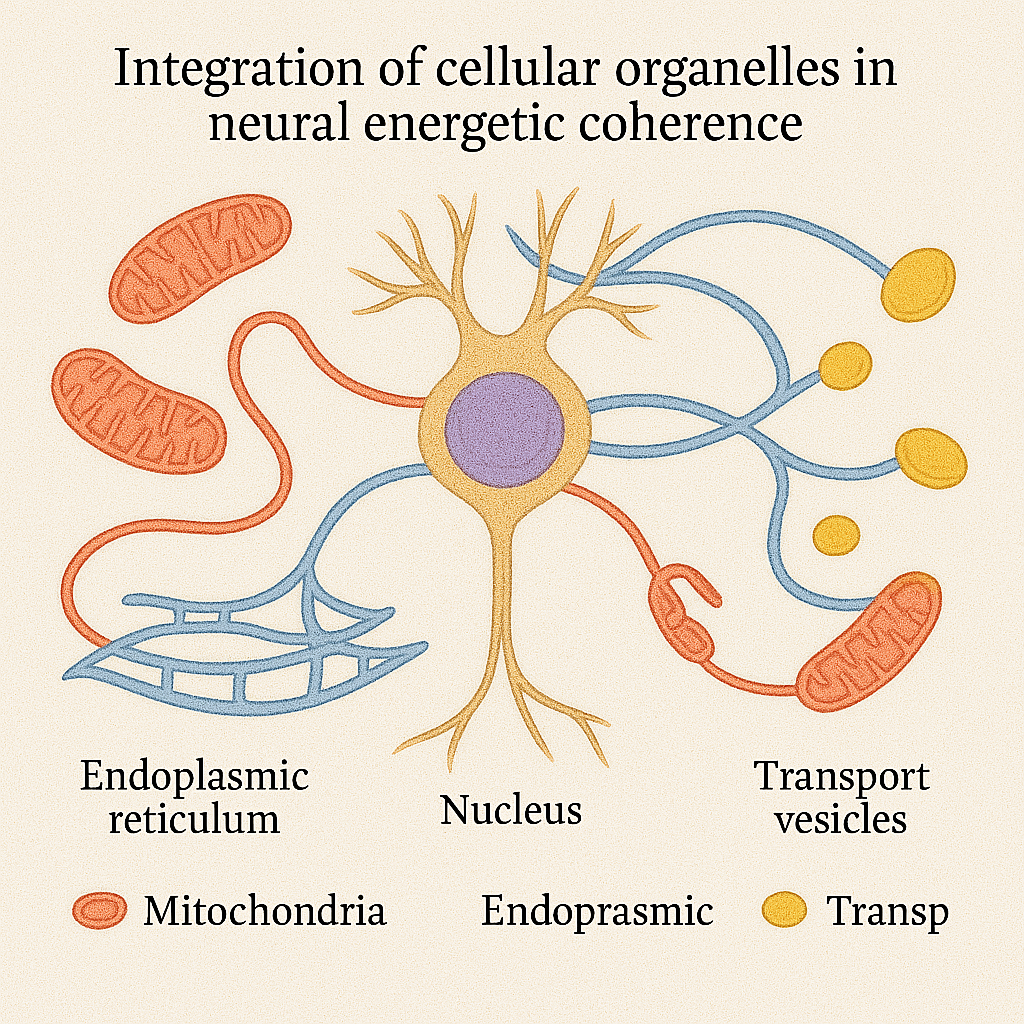
\includegraphics[width=0.8\textwidth]{images/cellular_organelles.png}

%   \caption{Integration of cellular organelles in neural energetic coherence. This illustration shows how different organelles coordinate to create the energetic foundation for conscious processing. At the center, mitochondria (red) form dynamic networks that adapt to energy demands, with their membrane potentials creating coherent electromagnetic fields. The endoplasmic reticulum (blue) extends throughout the cell, forming specialized contacts with mitochondria to coordinate calcium signaling and protein production. The nucleus (purple) actively regulates gene expression in response to neural activity, while various transport vesicles (yellow) ensure precise distribution of proteins and receptors. This integrated system demonstrates how consciousness emerges not from isolated components but from the coordinated interactions of multiple organelles establishing patterns of energetic coherence across different spatial and temporal scales.}
% \end{figure}

\subsubsection{Dynamic Networks and Adaptive Energy Production~\index{mitochondrial dynamics}~\index{energy production}}

\index{mitochondrial dynamics}Mitochondrial dynamics—their continuous fusion, fission, and movement—provide sophisticated mechanisms for adapting energy production to changing neural demands~\cite{Bertholet2016, Sheng2012}. Rather than remaining static, these organelles form dynamic networks that can reconfigure in response to local activity patterns. This remarkable mobility enables neural cells to redirect energy resources while maintaining overall~\index{energetic coherence}coherent function. The coordination between mitochondrial positioning and cellular activity demonstrates how~\index{biological systems}biological systems achieve sophisticated~\index{energy management}energy management through physical reorganization rather than abstract control systems.

\subsubsection{Membrane Potential and Energy Storage~\index{mitochondrial membrane potential}~\index{energy storage}}

The~\index{mitochondrial membrane potential}mitochondrial membrane potential represents a direct manifestation of~\index{energy storage}energy storage in a form immediately relevant to~\index{ECC!principles}ECC's principles~\cite{Nicholls2000, Picard2018}. This voltage gradient across the inner mitochondrial membrane stores energy through a physical state rather than through abstract representations. The careful maintenance of this potential enables rapid energy mobilization while providing buffer capacity against fluctuating demands. The ability to store energy in this field-like state proves particularly significant for maintaining~\index{coherent states}coherent neural activity.

\subsubsection{Bioelectric Networks and Primitive Consciousness~\index{bioelectric networks}~\index{primitive consciousness}}

\index{bioelectric networks}Bioelectric mitochondrial networks may represent one of the most primitive implementations of consciousness-like phenomena within individual cells~\cite{Picard2015, Pokorný2012}. These networks create sophisticated patterns of~\index{coherent fields}coherent electromagnetic fields through the coordinated activity of hundreds to thousands of mitochondria functioning as an integrated system~\cite{Thar2004, De Ninno2021}. The resulting~\index{mitochondrial intelligence}electrical coherence domains implement rudimentary forms of~\index{information integration}information integration across subcellular spaces, potentially supporting primitive awareness at the cellular level~\cite{Baluška2020, McFadden2020}. Investigating these networks with techniques such as~\index{voltage-sensitive dyes}voltage-sensitive dyes,~\index{super-resolution microscopy}super-resolution microscopy, and~\index{computational modeling}computational modeling of field dynamics could reveal how mitochondrial~\index{field coherence}field coherence implements the same fundamental principles that ECC identifies in neural-level consciousness, but at a much simpler scale~\cite{Pokorný2014, Ivanov2021}. These investigations might reveal whether individual cells possess a minimal form of~\index{sentience}sentience—not the rich, reflective consciousness of multicellular organisms, but rather the most basic implementation of integrated information through~\index{coherent energy states}coherent energy states that represents the fundamental building block from which more complex forms of consciousness evolve.

\subsubsection{Calcium Dynamics and Redox Signaling~\index{calcium dynamics}~\index{redox signaling}}

\index{mitochondria}Mitochondria contribute directly to cellular~\index{information processing}information processing through their effects on~\index{calcium dynamics}calcium dynamics and~\index{redox signaling}redox signaling~\cite{Ichas1998, pinotsis2023cytoelectric}. These organelles sequester and release calcium ions in coordination with other cellular systems, helping establish the precise~\index{calcium dynamics}calcium patterns necessary for neural signaling. Additionally, mitochondrial regulation of~\index{redox state}redox state influences protein function throughout the cell, creating another mechanism for coordinating cellular activity. This integration of energetic and signaling functions demonstrates how~\index{biological systems}biological systems achieve sophisticated processing through multifunctional components.

\subsubsection{Field Effects and Energetic Coherence~\index{local field effects}~\index{electrical coherence}}

The role of mitochondria in maintaining~\index{coherent states}coherent states extends to their contribution to~\index{local field effects}local field effects within cells~\cite{hunt2024electromagnetic, Thar2004}. The electrical properties of mitochondrial membranes influence broader patterns of field coherence across cellular compartments. This physical influence helps establish the conditions necessary for~\index{information integration}information integration while ensuring balanced~\index{energy flows}energy flows throughout the cell. The resulting field effects contribute significantly to the patterns of~\index{energetic coherence}energetic coherence that ECC identifies as crucial for consciousness.

\subsubsection{Astrocytic Networks and Intercellular Coordination~\index{astrocytic networks}~\index{glial-neuronal interactions}}

\index{mitochondrial networks}Mitochondrial networks in astrocytes deserve particular attention for their role in supporting~\index{conscious processing}conscious processing~\cite{Stephen2014, Verkhratsky2018}. These extensive networks enable sophisticated coordination of energy production across substantial volumes of neural tissue. Through their integration with~\index{astrocytic networks}astrocytic processes, mitochondria help establish the energetic foundation for~\index{glial-neuronal interactions}glial-neuronal interactions while ensuring proper metabolic support for neural activity. The resulting energetic architecture proves essential for maintaining~\index{coherent states}coherent conscious states.

\subsection{\index{nucleus}Nucleus and Genetic Regulation: Dynamic Information Storage~\index{genetic regulation}~\index{information storage}}

The~\index{nucleus}cell nucleus serves as more than a static repository of genetic information; it actively participates in~\index{conscious processing}conscious processing through sophisticated regulation of~\index{gene expression patterns}gene expression in response to neural activity~\cite{Greenberg2014, Yap2017}. This dynamic relationship between nuclear function and cellular activity creates responsive systems that can adapt their properties while maintaining coherent operation. The resulting integration of genetic regulation with broader patterns of neural function proves essential for sustained~\index{conscious processing}conscious processing.

\subsubsection{Three-Dimensional Architecture and Spatial Organization~\index{spatial organization}~\index{nuclear territories}}

The~\index{spatial organization}spatial organization within the nucleus demonstrates remarkable sophistication in its contribution to neural function~\cite{Dekker2013, Misteli2007}. Chromosomes occupy distinct~\index{nuclear territories}territories, with active genes often relocating to specialized transcription factories during expression. This three-dimensional architecture enables efficient coordination of~\index{gene expression patterns}gene expression while ensuring proper regulation of cell-type-specific programs. The resulting molecular organization helps establish the conditions necessary for region-specific processing capabilities while maintaining overall neural coherence.

\subsubsection{Chromatin Dynamics and Epigenetic Regulation~\index{chromatin dynamics}~\index{epigenetic regulation}}

\index{chromatin dynamics}Chromatin dynamics—the continuous reorganization of DNA packaging—enables sophisticated regulation of~\index{gene expression patterns}gene expression in response to neural activity~\cite{Maze2015, Yap2017}. These epigenetic mechanisms allow cells to adapt their molecular properties while preserving essential aspects of their identity. The precise coordination between neural activity patterns and chromatin modifications helps ensure appropriate responses to changing computational demands. This dynamic regulation proves crucial for the long-term maintenance of~\index{coherent states}coherent conscious states.

\subsubsection{Energetic Requirements and Resource Management~\index{nuclear energetics}~\index{resource management}}

The energy requirements of nuclear function deserve particular attention for their contribution to cellular energetics~\cite{Wright2016, Buszczak2014}. Transcription, RNA processing, and nuclear transport all require substantial energy input, creating significant demands on cellular resources. The careful coordination between nuclear activity and energy availability enables cells to maintain appropriate~\index{gene expression patterns}gene expression while avoiding energetic depletion. This sophisticated energy management proves essential for supporting sustained~\index{conscious processing}conscious processing.

\subsubsection{Nucleocytoplasmic Transport and Information Flow~\index{nucleocytoplasmic transport}~\index{information flow}}

\index{nucleocytoplasmic transport}Nucleocytoplasmic transport—the regulated movement of molecules between nucleus and cytoplasm—creates another layer of control in neural function~\cite{Freibaum2015, Raices2017}. This bidirectional exchange enables the nucleus to respond to cellular activity while influencing cytoplasmic processes. The resulting integration of nuclear and cytoplasmic functions helps establish coherent cellular states while enabling dynamic adaptations to changing conditions. This coordination across compartments demonstrates how~\index{biological systems}biological systems achieve sophisticated regulation through structured communication rather than centralized control.

\subsection{Endoplasmic Reticulum: Protein Production and Calcium Regulation~\index{endoplasmic reticulum}~\index{protein production}}

The~\index{endoplasmic reticulum}endoplasmic reticulum (ER) extends throughout neural cells, creating a continuous network for protein synthesis, modification, and~\index{calcium storage}calcium storage~\cite{Ramirez2018, Park2008}. This elaborate organelle proves particularly significant for~\index{conscious processing}conscious processing through its contributions to~\index{calcium dynamics}calcium regulation and protein production. The precise organization of the ER enables sophisticated coordination of multiple cellular processes while maintaining the stability necessary for coherent function.

\subsubsection{Calcium Stores and Signaling Integration~\index{calcium stores}~\index{signaling integration}}

\index{calcium stores}ER calcium stores play a crucial role in neural signaling and~\index{information processing}information processing~\cite{Berridge2014, Patel2010}. Through coordinated release and reuptake of calcium ions, the ER helps establish complex patterns of~\index{calcium signaling}calcium signaling that integrate information across multiple timescales. This regulation proves particularly important for~\index{synaptic plasticity}synaptic plasticity and cellular adaptation to changing activity patterns. The sophisticated management of calcium dynamics through ER function demonstrates how~\index{biological systems}biological systems achieve~\index{information integration}information integration through physical processes rather than abstract computation.

\subsubsection{Protein Synthesis and Molecular Infrastructure~\index{protein synthesis}~\index{molecular infrastructure}}

The ER's role in~\index{protein synthesis}protein synthesis and~\index{protein folding}protein folding creates the foundation for maintaining the specialized molecular machinery necessary for~\index{conscious processing}conscious processing~\cite{Hetz2015, reid2015er}. Through careful quality control and sophisticated folding mechanisms, the ER ensures proper production of the membrane proteins, receptors, and signaling molecules that enable neural function. This molecular manufacturing capability proves essential for maintaining the specific molecular compositions required for different aspects of~\index{conscious processing}conscious processing.

\subsubsection{Unfolded Protein Response and Cellular Resilience~\index{unfolded protein response}~\index{cellular resilience}}

The~\index{unfolded protein response}unfolded protein response (UPR) demonstrates how the ER contributes to cellular resilience and long-term stability~\cite{Hetz2012, Marciniak2004}. This adaptive mechanism enables cells to maintain proper protein processing despite changing demands or stress conditions. The sophisticated regulation of ER function through the UPR helps ensure consistent production of essential proteins while preventing accumulation of misfolded molecules. This quality control system proves crucial for maintaining the molecular basis of~\index{coherent states}coherent conscious states.

\subsubsection{ER-Mitochondria Contacts and Organelle Communication~\index{ER-mitochondria contacts}~\index{organelle communication}}

\index{ER-mitochondria contacts}ER-mitochondria contact sites create specialized microdomains for coordinating multiple cellular processes~\cite{Rowland2012, Csordas2018}. These physical junctions enable direct communication between organelles, facilitating lipid transfer, calcium exchange, and coordination of energy production with protein synthesis. The resulting integration of organelle functions helps establish coherent cellular states while enabling efficient resource utilization. This physical coupling between different components of cellular machinery demonstrates how~\index{biological systems}biological systems achieve sophisticated coordination through structured organization rather than abstract control systems.

\subsection{Additional Organelles and Support Systems~\index{cellular support systems}}

\subsubsection{Golgi Apparatus and Protein Distribution~\index{golgi apparatus}~\index{protein distribution}}

\index{golgi apparatus}The Golgi apparatus serves as a crucial processing and distribution center for cellular proteins~\cite{Nakamura2012, Ramirez2018}. Through sophisticated sorting mechanisms, this organelle directs newly synthesized proteins to their proper destinations within the cell. The precise organization of the Golgi enables cells to maintain appropriate distributions of membrane proteins, receptors, and other molecular components. This spatial control proves essential for establishing the specific patterns of molecular organization necessary for different aspects of~\index{conscious processing}conscious processing.

\subsubsection{Lysosomes and Quality Control~\index{lysosomes}~\index{quality control}}

\index{lysosomes}Lysosomes contribute to~\index{conscious processing}conscious processing through their role in cellular maintenance and~\index{protein turnover}protein turnover~\cite{Ferguson2012, Settembre2013}. These degradative organelles remove damaged proteins and cellular components, helping maintain proper function despite continuous use. The sophisticated regulation of lysosomal activity enables cells to adjust their maintenance processes based on current conditions and functional demands. This adaptive quality control proves crucial for sustaining~\index{coherent states}coherent conscious states across extended periods.

\subsubsection{Peroxisomes and Metabolic Support~\index{peroxisomes}~\index{metabolic support}}

\index{peroxisomes}Peroxisomes play specialized roles in lipid metabolism and~\index{redox regulation}redox regulation that support neural function~\cite{Fransen2012, Smith2013}. These small but essential organelles help maintain proper membrane composition while protecting cells from oxidative damage. The careful coordination between peroxisomal activity and broader cellular functions enables neural systems to maintain appropriate molecular conditions for~\index{information processing}information processing. This supportive role demonstrates how even seemingly peripheral organelles contribute significantly to the conditions necessary for~\index{conscious processing}conscious processing.

\subsubsection{Vesicular Transport and Molecular Trafficking~\index{vesicular transport}~\index{molecular trafficking}}

\index{vesicular transport}Vesicular transport systems create dynamic pathways for moving materials throughout neural cells~\cite{Bonanomi2006, Sudhof2004}. These sophisticated trafficking mechanisms enable precise delivery of molecular components to specific cellular locations, from synaptic terminals to dendritic spines. The resulting spatial control enables cells to maintain appropriate distributions of receptors, channels, and other functional proteins. This dynamic organization proves essential for establishing the specific patterns of molecular architecture necessary for~\index{conscious processing}conscious processing.

\subsubsection{Endosomal System and Membrane Regulation~\index{endosomal system}~\index{membrane regulation}}

\index{multivesicular bodies}Multivesicular bodies and~\index{endosomal system}the broader endosomal system contribute to neural function through regulation of membrane protein turnover and signaling~\cite{Huotari2011, Cosker2014}. These organelles enable sophisticated control over receptor expression and trafficking, helping cells adjust their response properties based on activity patterns. The resulting regulation of membrane composition proves crucial for maintaining appropriate sensitivity to incoming signals while avoiding pathological states of over- or under-activation.

\subsection{Integrated Organelle Function and Emergent Properties~\index{integrated function}~\index{emergent properties}}

\subsubsection{Inter-Organelle Communication Networks~\index{inter-organelle communication}~\index{cellular networks}}

The integration of organelle functions across neural cells reveals sophisticated principles of cellular organization~\cite{Valm2017, Vance2012}. Rather than operating independently, different organelles maintain continuous communication and coordination through both physical contacts and signaling pathways. This inter-organelle cooperation enables cells to maintain coherent function while adapting to changing conditions. The resulting cellular architecture demonstrates how~\index{biological systems}biological systems achieve sophisticated~\index{information processing}information processing through distributed yet integrated components.

\subsubsection{Three-Dimensional Organization and Resource Efficiency~\index{three-dimensional organization}~\index{resource efficiency}}

The spatial organization of organelles within neural cells demonstrates remarkable precision in supporting~\index{information processing}information processing and energy management~\cite{Kapitein2015, Sheng2012}. Different compartments maintain specific distributions of organelles based on local functional requirements and resource demands. This three-dimensional architecture enables efficient resource utilization while ensuring proper support for different aspects of cellular function. The resulting spatial organization proves essential for establishing the conditions necessary for~\index{coherent states}coherent conscious states.

\subsubsection{Energetic Coordination and Balanced Flows~\index{energetic coordination}~\index{balanced flows}}

The energetic aspects of inter-organelle communication deserve particular attention for their contribution to cellular coherence~\cite{Picard2018, Ramirez2018}. Through coordinated regulation of~\index{energy production}energy production, distribution, and utilization, organelles help establish balanced energy flows throughout neural cells. This energetic coordination enables cells to maintain stable function while responding effectively to changing demands. The resulting patterns of energy management demonstrate how~\index{biological systems}biological systems achieve the specific conditions necessary for~\index{conscious processing}conscious processing.

\subsubsection{Dynamic Adaptation and Flexible Stability~\index{dynamic adaptation}~\index{flexible stability}}

The dynamic nature of organelle interactions enables neural cells to adapt their properties while maintaining coherent function~\cite{Schuck2009, Rambold2015}. Through continuous regulation of organelle size, position, and activity, cells can adjust their processing capabilities in response to changing conditions. This adaptive organization creates flexible yet stable cellular systems capable of supporting diverse forms of neural computation. The sophisticated coordination of organelle dynamics demonstrates how~\index{biological systems}biological systems achieve~\index{coherent states}coherent states through physical reorganization rather than abstract control mechanisms.

\subsubsection{Network-Level Implications~\index{network implications}~\index{neural networks}}

The implications of integrated organelle function extend beyond individual cells to shape how neural networks maintain~\index{coherent states}coherent conscious states~\cite{Harris2012, Verkhratsky2018}. The cellular architecture established through coordinated organelle function creates the foundation for reliable neural signaling and network operation. This fundamental organization enables neural systems to perform complex computations while maintaining the stability necessary for~\index{conscious processing}conscious processing.

\subsubsection{ECC Principles and Biological Implementation~\index{ECC!biological implementation}~\index{biological consciousness}}

Perhaps most significantly, the study of cellular organelles through~\index{ECC!principles}ECC's framework reveals consciousness as emerging from remarkably sophisticated patterns of biological organization rather than abstract computation~\cite{Baluska2016, butlin2023consciousnessartificialintelligenceinsights}. The precise coordination of organelle functions across multiple scales creates the conditions necessary for~\index{coherent states}coherent conscious processing while enabling dynamic adaptation to changing demands. This understanding suggests new approaches to both investigating consciousness and developing therapeutic interventions for neurological disorders.

\subsubsection{Multi-Scale Integration and Conscious Experience~\index{multi-scale integration}~\index{conscious experience}}

The integrated function of cellular organelles demonstrates how~\index{consciousness}consciousness emerges not from single components but from precisely orchestrated interactions across multiple biological scales. From the molecular precision of protein folding in the ER to the energetic foundation established by mitochondrial networks, from the transcriptional regulation in the nucleus to the quality control provided by lysosomes—these diverse processes converge to create the specific patterns of~\index{energetic coherence}energetic coherence that consciousness requires. This remarkable biological architecture, refined through evolution to support both stable conscious states and flexible adaptation to changing demands, reveals fundamental principles about how physical systems can achieve the coherent yet dynamic processing that defines conscious experience. 

\subsection{Hierarchical Consciousness: From Cellular to Trans-Cellular Integration~\index{hierarchical consciousness}~\index{trans-cellular integration}}

\subsubsection{Biological Scale and Conscious Complexity~\index{biological scale}~\index{conscious complexity}}

The examination of cellular organelles and their integrated functions raises profound questions about the hierarchical nature of~\index{consciousness}consciousness across biological scales~\cite{Baluska2016, Dehaene2014}. While human-like consciousness clearly transcends individual cells, operating through the coordination of billions of neurons and glial cells, the sophisticated organization observed within single cells suggests the possibility of primitive forms of consciousness even at the cellular level—a perspective aligned with certain forms of~\index{biopsychism}biopsychism~\cite{Tononi2016, Feinberg2016}.

\subsubsection{Mathematical Boundary Conditions~\index{mathematical boundary conditions}~\index{threshold conditions}}

The~\index{mathematical framework}mathematical framework of~\index{energetic coherence}energetic coherence described in previous chapters provides crucial insight into what distinguishes these potential levels of consciousness and establishes the boundary conditions determining what gets integrated into trans-cellular awareness and what remains below the threshold of detection~\cite{Tononi2008, butlin2023consciousnessartificialintelligenceinsights}. The mathematical formalism of~\index{information integration}information integration through~\index{coherent energy states}coherent energy states helps define which patterns achieve sufficient coherence amplitude to contribute to higher-order conscious experience.

\subsubsection{Cellular-Level Coherent States~\index{cellular-level coherence}~\index{subcellular processing}}

Within individual cells, complex processes maintain their own patterns of~\index{coherent energy states}coherent energy dynamics—from~\index{mitochondrial networks}mitochondrial networks coordinating~\index{ATP (adenosine triphosphate)}ATP production to the~\index{endoplasmic reticulum}endoplasmic reticulum regulating~\index{calcium dynamics}calcium flows~\cite{Hameroff2014, McFadden2020}. These cellular-level coherent states implement sophisticated~\index{information processing}information processing that maintains cellular function, potentially constituting a primitive form of awareness at the unicellular scale. However, these cellular-level coherent states typically operate below the threshold required for integration into the broader field of trans-cellular consciousness that defines human experience.

\subsubsection{Threshold Requirements for Consciousness~\index{threshold requirements}~\index{conscious integration}}

The~\index{mathematical boundary conditions}mathematical boundary conditions established by~\index{ECC!principles}ECC's principles determine which patterns of~\index{coherent energy states}coherent energy flow achieve sufficient amplitude and spatiotemporal extension to contribute to trans-cellular consciousness~\cite{breakspear2005dynamics, gershman2023molecular}. These conditions include minimum thresholds for:

\begin{itemize}
\item Coherence amplitude that exceeds baseline metabolic fluctuations
\item Spatiotemporal extension across multiple cellular units
\item Stability duration that allows integration with other conscious contents
\item Coupling strength with established~\index{coherent states}coherent fields
\end{itemize}

\subsubsection{Physical Substrate for Trans-Cellular Integration~\index{physical substrate}~\index{trans-cellular coherence}}

The~\index{gap junctions}gap junction networks,~\index{astrocytic networks}astrocytic syncytia, and~\index{neural architecture}neural architectural features described in previous sections create the physical substrate that enables patterns of~\index{energetic coherence}energetic coherence to transcend individual cells and achieve trans-cellular integration~\cite{Yuste2020, hunt2024electromagnetic}. These structures establish domains where coherent states can propagate across cellular boundaries, creating the conditions necessary for human-like consciousness to emerge.

\subsubsection{Consciousness as a Spectrum~\index{consciousness spectrum}~\index{awareness gradients}}

This perspective suggests consciousness exists across a spectrum rather than as a binary phenomenon~\cite{Feinberg2016, barrett2017emotions}. From the primitive awareness potentially present in individual cells to the rich conscious experience of humans, what differs is the scale, complexity, and integration of~\index{coherent energy states}coherent energy states. The mathematical formalism of~\index{ECC!principles}ECC provides a unified framework for understanding this hierarchy, with the same fundamental principles—coherent energy dynamics implementing information integration—operating across all scales.

\subsubsection{Implications for Artificial Consciousness~\index{artificial consciousness}~\index{consciousness implementation}}

The relationship between cellular and trans-cellular consciousness reveals fascinating possibilities for understanding both biological consciousness and potential artificial implementations~\cite{butlin2023consciousnessartificialintelligenceinsights, Dehaene2017}. If consciousness emerges from specific patterns of~\index{energetic coherence}energetic coherence rather than particular biological substrates, then any system capable of maintaining similar patterns could potentially support conscious states. However, the remarkable~\index{biological structures}biological architecture described throughout this chapter—from~\index{protein complexes}protein complexes to organelle networks, from cellular membranes to neural assemblies—represents evolutionary-refined solutions to the challenge of maintaining coherent conscious states within physical constraints.

\subsubsection{Resolving Contradictions in Consciousness Research~\index{consciousness research}~\index{theoretical integration}}

Understanding this hierarchical nature of consciousness helps resolve apparent contradictions in consciousness research~\cite{Tononi2016, Seth2023}. Rather than debating whether consciousness is localized to specific brain regions or distributed across networks, the~\index{ECC!principles}ECC framework suggests consciousness emerges at multiple scales simultaneously, with different aspects of experience implemented through patterns of coherence that span from subcellular processes to broad neural networks. The boundary between which coherent states contribute to conscious experience and which remain below awareness is not fixed but dynamically regulated through attention, arousal, and neuroplasticity.

\subsubsection{Evolutionary Perspective~\index{evolutionary perspective}~\index{consciousness evolution}}

This hierarchical perspective on consciousness also aligns with evolutionary considerations~\cite{Feinberg2016, gershman2023molecular}. The sophisticated integration mechanisms that support human consciousness likely evolved from simpler forms of coherence present in single-celled organisms and simple neural networks. The mathematical principles of~\index{energetic coherence}energetic coherence would have provided continuous selection pressure toward increasingly sophisticated forms of information integration and conscious experience throughout biological evolution.

\subsubsection{Practical Applications and Future Directions~\index{practical applications}~\index{future directions}}

The implications of this hierarchical understanding extend to both theoretical neuroscience and practical applications in medicine and technology~\cite{Dehaene2014, Seth2023}. By recognizing how different scales of coherent energy dynamics contribute to conscious experience, we gain new approaches to investigating~\index{disorders of consciousness}disorders of consciousness, developing more sophisticated~\index{brain-computer interfaces}brain-computer interfaces, and potentially creating artificial systems capable of supporting conscious-like states. 

Having explored the cellular foundations of consciousness through organelles and their integrated functions, we must now consider how these principles manifest at the systems level—how specialized neural circuits, brain regions, and global dynamics implement the energetically coherent computation that supports the rich tapestry of conscious experience. 